\section{Passphrase-protected private key(BIP38)}
BIP38提出了一种使用passphrase对私钥进行加密保护的方案。该方案只考虑了针对私钥的机密性保护,而没有考虑提供完整性保护,因此其主要针对纸钱包和physical Bitcoin等私钥密文不容易遭受篡改的应用场景。该协议主要提出了两种加密私钥的方法,其中一种方法使用了EC 乘法操作,另一种没有,从而导致两种方法实现的功能有很大的区别:
\begin{itemize}
\item Encryption when EC multiply is not used: 对于已经产生的私钥,使用用户设置的passphrase对私钥进行加密。加密后的密文与passphrase在解密私钥时缺一不可,由于两者可以独立存储、传输,从而提高了私钥的安全性。
\item Encryption when EC multiply is used: 用户首先会生成一个intermediate passphrase code(包含一个由passphrase单向生成的椭圆曲线群上的点,以及用户产生的salt),并将其传输给一个第三方(由于该方案针对的场景主要是纸钱包,这里的第三方通常是一个printer),第三方可以为用户生成新的地址,并对恢复该地址对应私钥的必要信息加密后展示给用户。用户拿到密文解密后,结合passphrase,即可算出新地址对应的私钥。这种方式允许用户将生成新地址的工作委托给一个不那么可信的第三方来做,同时保证只有知道passphrase和密文的人才能计算出对应私钥。
\end{itemize}


\subsection{ 编码格式}
针对两种私钥加密方式,对私钥加密保护后的数据编码格式略有不同,但长度都是39字节。
\begin{itemize}
\item 对于不使用EC乘法的,最终的数据由对 $0x01$ $0x42+ flagbyte+ addrhash+ encryptedhalf1$ $+ encryptedhalf2$进行Base58Check编码后的数据构成。
而对于使用EC乘法的,加密保护后的私钥数据由$0x01$ $0x43+ flagbyte+ addrhash+ ownerentropy+ encryptedhalf1$ $+ encryptedhalf2$进行Base58Check编码后的数据构成(具体含义会在后面详细介绍)。

\item $0x01$ $0x42/43$是为了使经过Base58Check编码后的结果以$6P$开头,6代表了"a private key that needs something else to be usable",P代表了上一句中的"something is a passphrase"。

\item flagbyte为1字节,最高两位用来区分是否使用EC乘法:11表示不使用EC乘法,反之设置为00。$0x20$用来表示私钥转换成比特币地址时使用的是压缩公钥的格式。$0x40$用来表示在使用EC乘法时,同时也使用了lot+sequence,这两个数字的作用会在后面说明。$0x10,0x08$予以保留。

\item Addrhash为对比特币地址进行两次SHA256操作后,取前四个字节的结果。
\end{itemize}

\subsection{Encryption when EC multiply is not used}
该方法对已知的私钥进行加密,加密过程分为两部分:从passphrase使用Scrypt派生AES加密的密钥;使用AES对私钥信息进行加密。

\begin{algorithm}[tbp]\footnotesize
\caption{Encryption}\label{encryption without ec multiply}
  	\begin{algorithmic}[1]
	    \STATE Compute the Bitcoin address (ASCII), and take the first four bytes of $SHA256(SHA256())$ of it. Let's call this "addresshash".
		\STATE Derive a key from the passphrase using scrypt  
		
		\STATE Parameters: passphrase is the passphrase itself encoded in UTF-8 and normalized using Unicode Normalization Form C (NFC). salt is addresshash from the earlier step, $n=16384, r=8, p=8, length=64 $(n, r, p are provisional and subject to consensus)  
		\STATE Let's split the resulting 64 bytes in half, and call them derivedhalf1 and derivedhalf2
		\STATE Do $AES256Encrypt(block = bitcoinprivkey[0...15] \oplus derivedhalf1[0...15], key = derivedhalf2)$, call the 16-byte result encryptedhalf1  
		\STATE Do $AES256Encrypt(block = bitcoinprivkey[16...31] \oplus derivedhalf1[16...31], key = derivedhalf2)$, call the 16-byte result encryptedhalf2 
		\STATE The encrypted private key is the Base58Check-encoded concatenation of the following, which totals 39 bytes without Base58 checksum:$0x01$ $0x42 + flagbyte + salt + encryptedhalf1 + encryptedhalf2$
    \end{algorithmic}
\end{algorithm}

\begin{figure}[h]
\centering
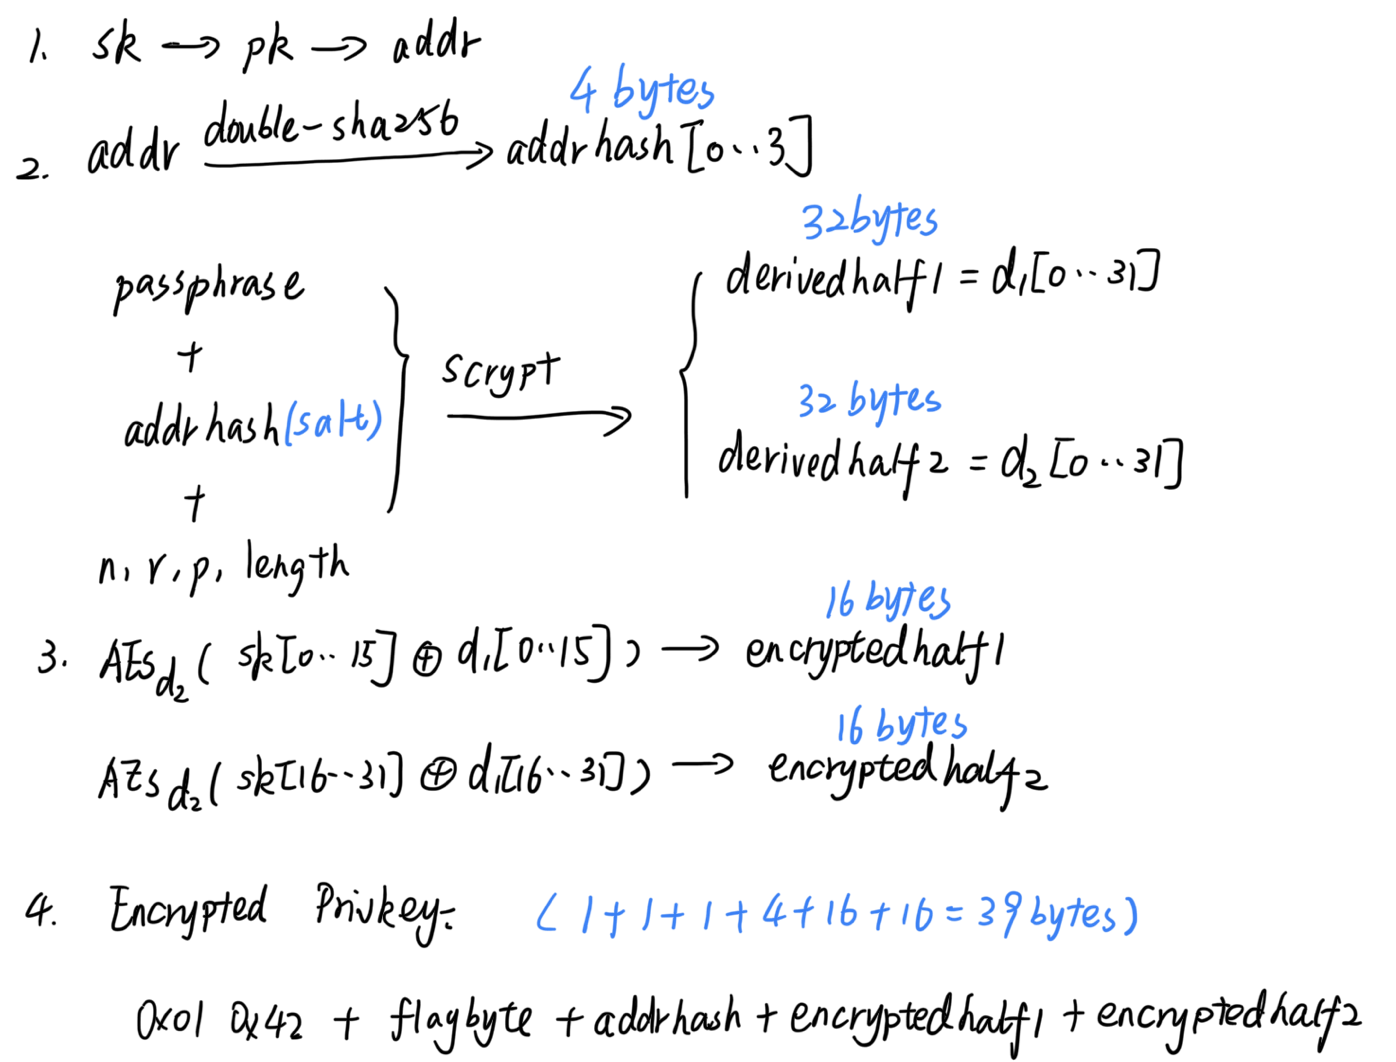
\includegraphics[width=.7\textwidth]{./no-ec.png}
\caption{caption}\label{fig-parsesig}
\end{figure}

在使用Scrypt派生密钥时,Scrypt参数中salt设置为比特币地址经过double-SHA256后的前4个字节。该字段无需保密,目的是为了增加攻击者进行暴力破解时的搜索空间,增加攻击的时间/空间复杂度。



解密过程首先根据用户掌握的passphrase计算出AES的解密密钥,随后对密文解密:

\begin{algorithm}[tbp]\footnotesize
\caption{Decryption}
  	\begin{algorithmic}[1]
	    \STATE Collect encrypted private key and passphrase from user.  
		\STATE Derive derivedhalf1 and derivedhalf2 by passing the passphrase and addresshash into scrypt function.
		\STATE Decrypt encryptedhalf1 and encryptedhalf2 using AES256Decrypt, merge them to form the encrypted private key. 
		\STATE Convert that private key into a Bitcoin address, honoring the compression preference specified in flagbyte of the encrypted key record.
		\STATE Hash the Bitcoin address, and verify that addresshash from the encrypted private key record matches the hash. If not, report that the passphrase entry was incorrect.  
    \end{algorithmic}
\end{algorithm}


\subsection{Encryption when EC multiply is used}

该方法利用了EC 乘法的同态性质,主要思想类似于一个基于椭圆曲线的密钥协商方案:用户事先由passphrase和entropy等生成一个随机数x,并计算对应的椭圆曲线群上的点$P=x*G$,将其发给第三方。随后,第三方选择一个随机数k与该点进行EC的乘法操作,即视为新生成的公钥$P'=k*P=(x \cdot k)*G$。随后将k加密后发送给用户(加密过程与上一个方法类似)。用户收到数据解密后,计算出新私钥$x\cdot k$。假设用于生成x的passphrase被保护的足够好,那么用户就可以确认新私钥是足够安全的(只有掌握passphrase的人才能计算),这一点可以认为是使用该方法生成新的加密私钥所额外带来的一个安全性方面的好处。
该算法包含两个阶段:初始化阶段、私钥生成阶段。

\subsubsection{初始化}
初始化阶段主要功能是用户由passphrase和ownerentrpy计算intermediate passphrase code,并发送给第三方。  

在计算时,用户可以选择性的生成一个20bit的lot number和12bit的sequence number。在用户向第三方请求大量的加密私钥时,需要检查返回的私钥对应的lot和sequence number是否与他所提供的intermediate passphrase code一致,以防止来自第三方的潜在攻击。这4字节lot+sequence number并不是必须的,在两种场景下,初始化阶段稍微不同。 
 
在使用lot+sequence时:  

\begin{algorithm}[tbp]\footnotesize
\caption{Initialize with lot sequence}
  	\begin{algorithmic}[1]
	    \STATE Generate 4 random bytes, call them ownersalt. 
		\STATE Encode the lot and sequence numbers as a 4 byte quantity (big-endian): $lotnumber * 4096 + sequencenumber$. Call these four bytes lotsequence.
		\STATE Derive a key from the passphrase using scrypt. 
		\STATE Parameters: passphrase is the passphrase itself encoded in UTF-8 and normalized using Unicode Normalization Form C (NFC). salt is ownersalt. $n=16384, r=8, p=8, length=32$.
		\STATE Call the resulting 32 bytes prefactor.
		\STATE Take $SHA256(SHA256(prefactor + ownerentropy))$ and call this passfactor. The "+" operator is concatenation.
		\STATE Compute the elliptic curve point $G * passfactor$, and convert the result to compressed notation (33 bytes). Call this passpoint. Compressed notation is used for this purpose regardless of whether the intent is to create Bitcoin addresses with or without compressed public keys.
		\STATE Convey ownersalt and passpoint to the party generating the keys, along with a checksum to ensure integrity.
		\STATE The following Base58Check-encoded format is recommended for this purpose: magic bytes "2C E9 B3 E1 FF 39 E2 51" followed by ownerentropy, and then passpoint. The resulting string will start with the word "passphrase" due to the constant bytes, will be 72 characters in length, and encodes 49 bytes (8 bytes constant + 8 bytes ownerentropy + 33 bytes passpoint). The checksum is handled in the Base58Check encoding. The resulting string is called "intermediate_passphrase_string".

    \end{algorithmic}
\end{algorithm}


\begin{figure}[h]
\centering
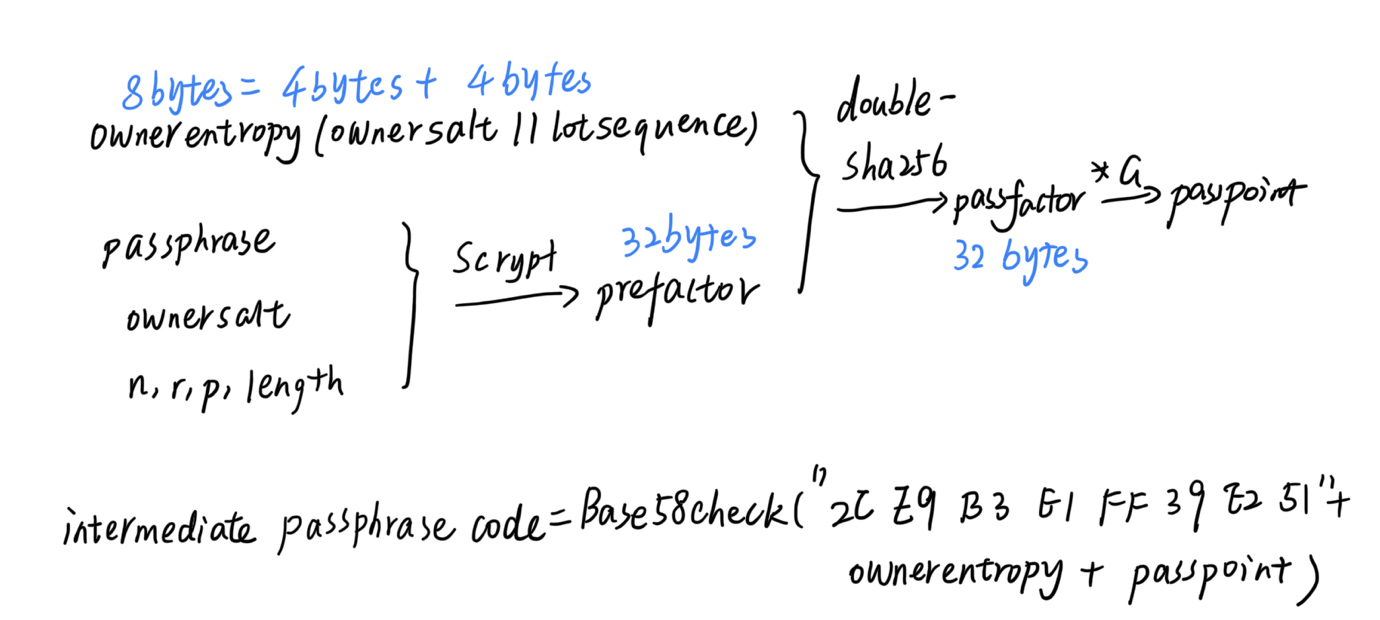
\includegraphics[width=.7\textwidth]{./im-code1.png}
\caption{caption}\label{fig-parsesig}
\end{figure}

\begin{algorithm}[tbp]\footnotesize
\caption{Initialize without lot sequence}
  	\begin{algorithmic}[1]
	    \STATE ownersalt is 8 random bytes instead of 4, and lotsequence is omitted. ownerentropy becomes an alias for ownersalt. 
		\STATE The SHA256 conversion of prefactor to passfactor is omitted. Instead, the output of scrypt is used directly as passfactor.
		\STATE The magic bytes are "2C E9 B3 E1 FF 39 E2 53" instead (the last byte is 0x53 instead of 0x51). 
    \end{algorithmic}
\end{algorithm}



\begin{figure}[h]
\centering
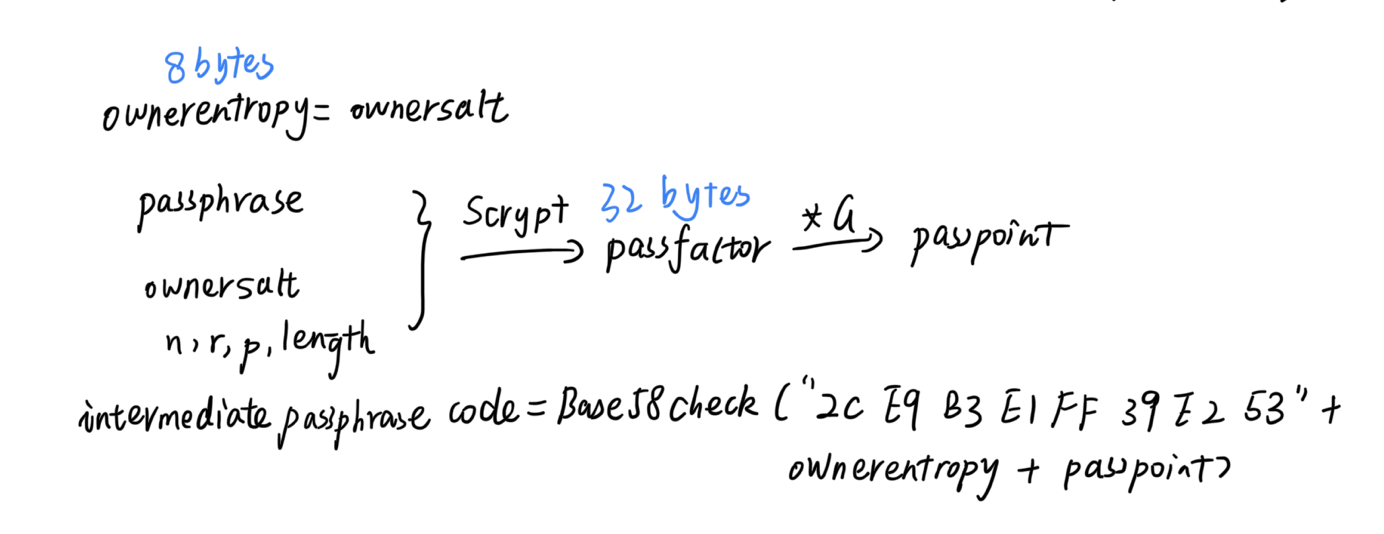
\includegraphics[width=.7\textwidth]{./im-code2.png}
\caption{caption}\label{fig-parsesig}
\end{figure}

\subsubsection{加密私钥计算}
第三方拿到intermediate passphrase code后,可以用它为用户生成新的加密私钥。确切地说,
第三方可以为用户生成新的公钥,并将计算对应私钥的所需的必要信息进行加密,
同时拥有passphrase和该密文人才能从中计算出对应的私钥。  
计算过程如下:

\begin{algorithm}[tbp]\footnotesize
\caption{New Public Key Generation}
  	\begin{algorithmic}[1]
	    \STATE Set flagbyte.
	    \STATE Turn on bit 0x20 if the Bitcoin address will be formed 
	    by hashing the compressed public key (optional). Turn on bit 0x04 
	    if ownerentropy contains a value for lotsequence.   
		\STATE Generate 24 random bytes, call this seedb. 
		Take $SHA256(SHA256(seedb))$ to yield 32 bytes, call this factorb.
		\STATE ECMultiply passpoint by factorb. Use the resulting EC point 
		as a public key and hash it into a Bitcoin address using either 
		compressed or uncompressed public key methodology. 
		This is the generated Bitcoin address, call it generatedaddress. 
    \end{algorithmic}
\end{algorithm}

以上完成了新公钥(passpoint*factorb)的生成过程。以下过程即是加密过程,与encryption when EC multiply is not used的过程类似。即由passpoint和salt派生AES的加密密钥,然后对新公钥对应私钥的部分信息(seedb)进行加密。

\begin{algorithm}[tbp]\footnotesize
\caption{Encryption}
  	\begin{algorithmic}[1]
	    \STATE Take the first four bytes of SHA256(SHA256(generatedaddress)) 
	    and call it addresshas
	    \STATE Now we will encrypt seedb. Derive a second key from passpoint 
	    using scrypt 
		\STATE Parameters: passphrase is passpoint provided from the first 
		party (expressed in binary as 33 bytes). 
		salt is addresshash + ownerentropy, $n=1024, r=1, p=1, length=64$. 
		The "+" operator is concatenation.
		\STATE Split the result into two 32-byte halves and call them derivedhalf1 
		and derivedhalf2.
		\STATE Do $AES256Encrypt(block = (seedb[0...15] \oplus derivedhalf1[0...15]), 
		key = derivedhalf2)$, call the 16-byte result encryptedpart1
		\STATE Do $AES256Encrypt(block = ((encryptedpart1[8...15] + seedb[16...23]) 
		\oplus derivedhalf1[16...31]), key = derivedhalf2)$, call the 16-byte result 
		encryptedpart2. The "+" operator is concatenation.
		\STATE The encrypted private key is the Base58Check-encoded concatenation of 
		the following, which totals 39 bytes without Base58 checksum: 
		$$0x01 0x43 + flagbyte + addresshash + ownerentropy +  encryptedpart1[0...7] + 
		encryptedpart2$$
    \end{algorithmic}
\end{algorithm}

这里最终数据的格式略有些奇怪,猜想是为了与不使用EC乘法的结果长度保持一致。相比较,这里比前面多了一个
8字节的ownerentroy字段,因此选取的seedb长度也就限制在了24字节。

\begin{figure}[h]
\centering
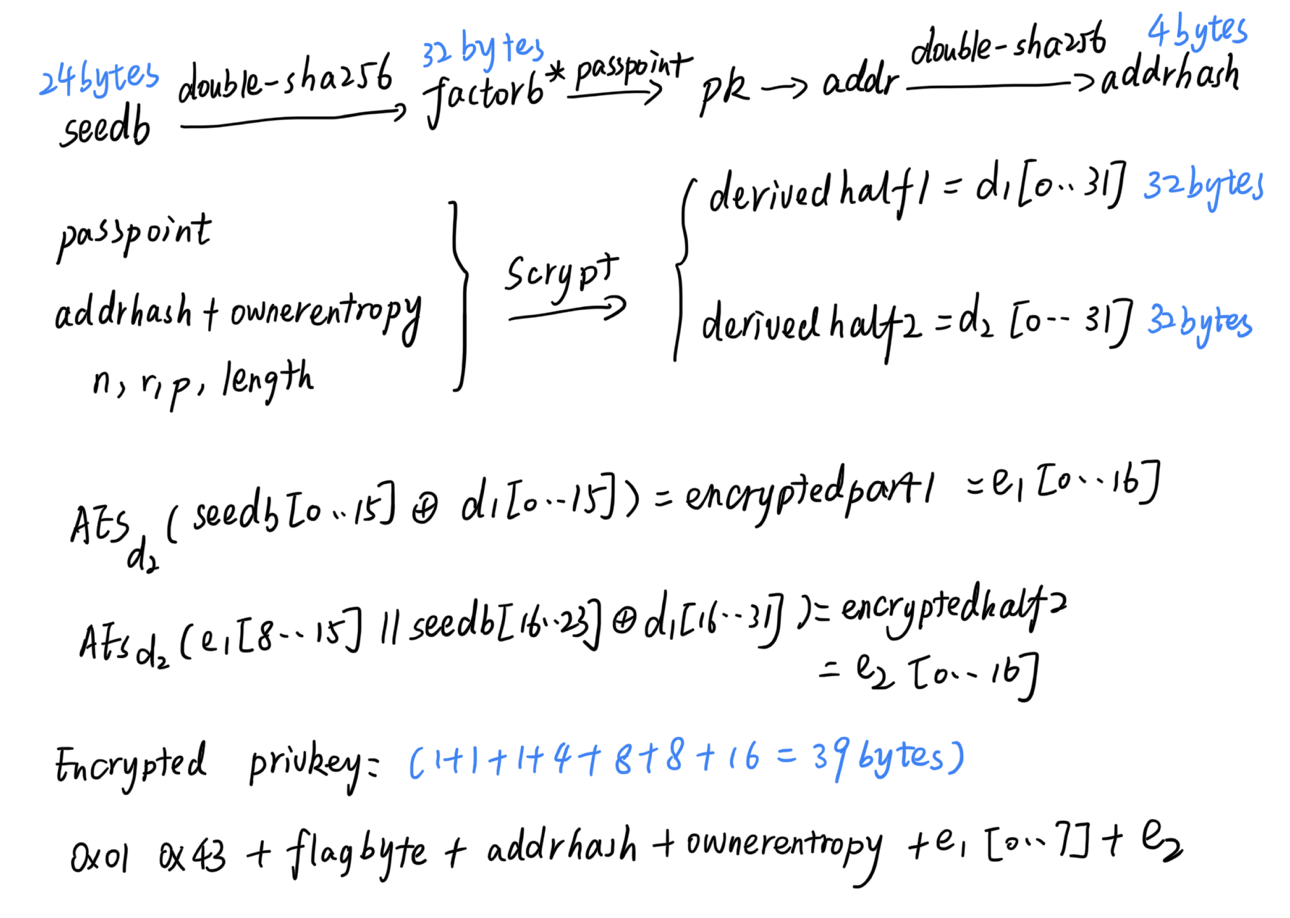
\includegraphics[width=.7\textwidth]{./ec.png}
\caption{caption}\label{fig-parsesig}
\end{figure}

\subsubsection{恢复新私钥}
从第三方返回的密文计算新私钥的过程如下(通常也是由客户端替用户计算的):

\begin{algorithm}[tbp]\footnotesize
\caption{Decryption and Private Key Computation}
  	\begin{algorithmic}[1]
	   \STATE  Collect encrypted private key and passphrase from user.
	   \STATE  Derive passfactor using scrypt with ownersalt and the user's 
	   passphrase and use it to recompute passpoint
	   \STATE Derive decryption key for seedb using scrypt with passpoint, 
	   addresshash, and ownerentropy
		\STATE Decrypt encryptedpart2 using AES256Decrypt to yield the last 
		8 bytes of seedb and the last 8 bytes of encryptedpart1.
		\STATE Decrypt encryptedpart1 to yield the remainder of seedb.
		\STATE Use seedb to compute factorb.
		\STATE Multiply passfactor by factorb mod N to yield the private key 
		associated with generatedaddress.
		\STATE C\STATE onvert that private key into a Bitcoin address, honoring 
		the compression preference specified in the encrypted key.
		\STATE Hash the Bitcoin address, and verify that addresshash from the 
		encrypted private key record matches the hash. If not, report that the 
		passphrase entry was incorrect.
    \end{algorithmic}
\end{algorithm}

以上过程完成了从密文中恢复seedb,以及从seedb计算factorb的过程。由于新公钥为$passpoint\cdot 
factorb=passfactor\cdot factorb *G$,对应的私钥即为$passfactor\cdot factorb$。

在恢复了新私钥后,客户端还需要验证计算出的私钥与之前addresshash给出的地址是否对应,如果不是,
则需要向用户返回错误信息,即用户输入了错误的passphrase。(由于该协议描述的目的场景是针对纸钱包,
所以可以假定上述编码后的密文的完整性是可以保证的,不会被篡改。)


\subsubsection{ Confirmation Code}
在printer为用户生成新的加密后的私钥后,用户当时可能并不需要进行解密(私钥只有在花费对应地址的UTXO时才需要),
但他需要对产生的新地址进行确认,以防自己使用的地址对应的私钥并不是自己可计算的。因此,对于使用EC multiply加密私钥的方式,该协议还设计了一个独立的验证方式,即printer可以向用户返回一个以“cfrm38”开头的
75个字符的confirmation code,用来协助用户验证新地址是否是自己可计算的。
 
Confirmation code生成过程如下:

\begin{algorithm}[tbp]\footnotesize
\caption{Confirmation Code}
  	\begin{algorithmic}[1]
	   \STATE To generate it, we need flagbyte, ownerentropy, factorb, derivedhalf1 and 
	   derivedhalf2 from the original encryption operation.
		\STATE ECMultiply factorb by G, call the result pointb. The result is 33 bytes.
		\STATE The first byte is 0x02 or 0x03. XOR it by (derivedhalf2[31] \& 0x01), call 
		the resulting byte pointbprefix.
		\STATE Do $AES256Encrypt(block = (pointb[1...16] \oplus derivedhalf1[0...15]), 
		key = derivedhalf2)$ and call the result pointbx1.
		\STATE Do $AES256Encrypt(block = (pointb[17...32] \oplus derivedhalf1[16...31]),
		 key = derivedhalf2)$ and call the result pointbx2.
		\STATE Concatenate pointbprefix + pointbx1 + pointbx2 (total 33 bytes) 
		and call the result encryptedpointb.  
		\STATE The result is a Base58Check-encoded concatenation of the following: \\ 
		 $0x64$ $0x3B$ $0xF6$ $0xA8$ $0x9A$ + $flagbyte + addresshash + ownerentropy + 
		 encryptedpointb$
    \end{algorithmic}
\end{algorithm}

除了常数部分,Confirmation code与私钥密文数据的不同之处在于encryptedpointb,
其中包含了$factor*G$的信息,允许用户收到confirmation code后计算出地址,
进行两次SHA256后去前四个字节与addresshash进行比对验证。
如果验证通过,用户可以使用该地址进行交易,且可以在进行花费时再解密相应私钥。

验证过程如下:

\begin{algorithm}[tbp]\footnotesize
\caption{Confirmation}
  	\begin{algorithmic}[1]
	   \STATE Derive passfactor using scrypt with ownerentropy and 
	   the user's passphrase and use it to recompute passpoint
		\STATE Derive decryption key for pointb using scrypt with 
		passpoint, addresshash, and ownerentropy
		\STATE Decrypt encryptedpointb to yield pointb
		\STATE ECMultiply pointb by passfactor. Use the resulting 
		EC point as a public key and hash it into address using either 
		compressed or  uncompressed public key methodology as specifid in flagbyte.
    \end{algorithmic}
\end{algorithm}


\subsubsection{ Security issues}

Confirmation code存在一个安全隐患:仅仅靠4bytes的addresshash来关联
confirmation code和encrypted key是不够的。一个不诚实的printer可以提供两个不同的factorb,
同时它们能够产生经过double-sha256后前32bit相同的两个地址。这时,仅仅验证confirmation code是不能够保证用户一定能够计算出他使用的地址所对应的私钥的。
这也就是说,confirmation code并不能起到他所声称的作用。
比如,printer计算出seedb1以及相应的factorb1,并计算出新私钥对应的地址addr1、
$addrhash1=SHA256(SHA256(addr1))_{4bytes}$。由于addrhash只有4字节,他可以遍历factorb的取值,
直到找到addrhash2=addrhash1的factorb2(计算复杂度为$O(2^{16})$)。这时,他就可以根据seedb1来计算encrypted key,根据factorb2来构造confirmation code,并且encrypted key和confirmation 
code中的addrhash是相同的。之后,将confirmation code和encrypted key发给用户。用户验证confirmation code可以通过,并使用其中计算出的addr2来收款,但是他无法计算出addr2对应的私钥(用户只知道factorb2*G的值),
他从encrypted key中计算出来的私钥对应于 $factorb1 * passfactor$,所以addr2中的钱将无法被花费。

在新私钥的生成中,存在一个安全隐患:在同一个intermediate passphrase code下,如果printer知道了其中一个加密私钥的明文,那么它就可以绕开用户的passphrase,
得到在当前intermediate passphrase code下派生的所有私钥。
 对于intermediate passphrase code $ipc1$,printer生成了一个随机数seedb1,
 按照以上计算(EC multiply used),生成的新私钥应该是$k1=passfactor * factorb1$ 
 $mod n$, $factorb1=SHA256(SHA256(seedb1))$。 假如printer知道了该私钥k1,他就可以计算 
 $passfactor=k1 * factorb1^{-1}$ $mod$ $n$, 因此,在同一个ipc1下的所有私钥都可以被printer计算出来。  
这种场景是存在的:如用户委托printer为自己生成新的加密私钥后,不小心又委托他对该私钥按照本协议第一种方法
(with no EC multiply)进行加密,恶意的printer可以检测到该私钥是它之前按照第二种方法生成的(对比公钥或地址),
这时它就具备了以上攻击的条件。

\begin{lstlisting}[language=python, caption = 测试代码, label=lst-baddersig]

import hashlib 
import secrets
from Crypto.Cipher import AES
import base58check
import scrypt
from bitcoinlib.keys import *
import ecdsa
from ecdsa.curves import SECP256k1
from ecdsa.ecdsa import int_to_string, string_to_int

# parameter for Scrypt function
SCRYPT_N=16384
SCRYPT_R=8
SCRYPT_P=8

def b58check(data):
	# return base58 encoding of data with checksum
	checksum=hashlib.sha256(data).digest()
	checksum=hashlib.sha256(checksum).digest()
	data+=checksum[:4]
	return base58check.b58encode(data)
\end{lstlisting}

\begin{lstlisting}[language=python, caption = Encryption \& Decryption with no EC multiplication,
 label=lst-baddersig]

def enc_without_ec_multi(privkey,address,passphrase,compressed):
	# compute addrhash of corresponding address to known private key
	addrhash=hashlib.sha256(address).digest()
	addrhash=hashlib.sha256(addrhash).digest()
	addrhash=addrhash[:4]
	# derive encryption key for AES
	passphrase=passphrase.decode('utf-8')
	d=scrypt.hash(passphrase,addrhash,SCRYPT_N,SCRYPT_R,SCRYPT_P,64)
	derivedhalf1=d[:32]
	derivedhalf2=d[32:64]
	# encryption process
	m1=[a^b for a,b in zip(privkey[:16],derivedhalf1[:16])]
	m2=[a^b for a,b in zip(privkey[16:32],derivedhalf1[16:32])]
	e1=AES.new(derivedhalf2).encrypt(bytes(m1))
	e2=AES.new(derivedhalf2).encrypt(bytes(m2))
   # pack encryption data
	flagbyte=b'\xe0' if compressed==1 else b'\xC0'
	res=b'\x01\x42'+flagbyte+addrhash+e1+e2
	return b58check(res)
	
def dec_without_ec_multi(encrypted_privkey,passphrase):
	# unpack data 
	data=base58check.b58decode(encrypted_privkey)
	addrhash_v=data[3:7]
	passphrase=passphrase.decode('utf-8')
	# derive decryption key for AES
	d=scrypt.hash(passphrase,addrhash_v,SCRYPT_N,SCRYPT_R,SCRYPT_P,64)
	derivedhalf1=d[:32]
	derivedhalf2=d[32:64]
	# decryption process
	m1=AES.new(derivedhalf2).decrypt(data[7:23])
	m2=AES.new(derivedhalf2).decrypt(data[23:39])
	privkey1=bytes([a^b for a,b in zip(m1,derivedhalf1[:16])])
	privkey2=bytes([a^b for a,b in zip(m2,derivedhalf1[16:32])])
	privkey=privkey1+privkey2
	# verify whether addrhash is correct
	k=Key(privkey)
	addr=k.address_uncompressed() if data[2]==0xC0 else k.address()
	addrhash=hashlib.sha256(addr.encode('ascii')).digest()
	addrhash=hashlib.sha256(addrhash).digest()
	if addrhash!=addrhash_v:
		assert("address is not valid!")
	else:
		return privkey1+privkey2
\end{lstlisting}

\begin{lstlisting}[language=bash, caption = 测试结果 label=lst-baddersig]
Encryption with no EC multiplication:
Privkey is : b'\xcb\xf4\xb9\xf7\x04p\x85k\xb4\xf4\x0f\x80\xb8~\xdb\x90\x86Y\x97\xff\xeem\xf3\x15\xab\x16mq:\xf43\xa5'
Encrypted private key is : b'6PRVWUbkzzsbcVac2qwfssoUJAN1Xhrg6bNk8J7Nzm5H7kxEbn2Nh2ZoGg'

Decryption with no EC multiplication:
Decryption succeed!
Private key is  b'\xcb\xf4\xb9\xf7\x04p\x85k\xb4\xf4\x0f\x80\xb8~\xdb\x90\x86Y\x97\xff\xeem\xf3\x15\xab\x16mq:\xf43\xa5'
\end{lstlisting}

\begin{lstlisting}[language=python, caption = Encryption \& Decryption with EC mutiplication, 
label=lst-baddersig]
def init_enc_with_ec_multi(passphrase,ownersalt,lotsequence):
	if len(ownersalt+lotsequence)!=8:
		assert("ownerentropy must be 8 bytes!")
	# derive prefactor from scrypt
	prefactor=scrypt.hash(passphrase,ownersalt,SCRYPT_N,SCRYPT_R,SCRYPT_P,32)
	#derive passpoint & pack intermediate passphrase code
	if len(lotsequence)==0:
		intermediate_passphrase_code=b'\x2C\xE9\xB3\xE1\xFF\x39\xE2\x53'
		intermediate_passphrase_code+=ownersalt
		passfactor=prefactor
		print("ownersalt",ownersalt)
	else:
		intermediate_passphrase_code=b'\x2C\xE9\xB3\xE1\xFF\x39\xE2\x51'+ownersalt+lotsequence
		prefactor+=(ownersalt+lotsequence)
		passfactor=hashlib.sha256(prefactor).digest()
		passfactor=hashlib.sha256(passfactor).digest()
	k=Key(bytes(passfactor))
	passpoint=k.public_compressed_byte
	intermediate_passphrase_code+=passpoint
	return b58check(intermediate_passphrase_code)

def enc_with_ec_multi(intermediate_passphrase_code,flag_lotseq,flag_compr):	
	#unpack intermediate passphrase code
	intermediate_passphrase_code=base58check.b58decode(intermediate_passphrase_code)
	ownerentropy=intermediate_passphrase_code[8:16]
	passpoint=intermediate_passphrase_code[16:49]

	# generate random seedb to derive new public key & address
	seedb=secrets.token_bytes(24)
	factorb=hashlib.sha256(seedb).digest()
	factorb=hashlib.sha256(factorb).digest()
	k=Key(bytes(passpoint))
	(x,y)=k.public_point()
	c=ecdsa.ellipticcurve.CurveFp(SECP256k1.curve.p(),SECP256k1.curve.a(),SECP256k1.curve.b())
	p=ecdsa.ellipticcurve.Point(c,x,y)
	new_point=p.__mul__(string_to_int(factorb))
	k=Key(new_point.x()+new_point.y())
	addr=k.address() if flag_compr==1 else k.address_uncompressed()
	addrhash=hashlib.sha256(base58check.b58decode(addr)).digest()
	addrhash=hashlib.sha256(addrhash).digest()
	addrhash=addrhash[:4]

	# derive encryption key and use AES to encrypt seedb
	salt=addrhash[:4]+ownerentropy
	d=scrypt.hash(passpoint,salt,1024,1,1,64)
	derivedhalf1=d[:32]
	derivedhalf2=d[32:64]
	m1=[a^b for a,b in zip(seedb[:16],derivedhalf1[:16])]
	e1=AES.new(derivedhalf2).encrypt(bytes(m1))
	m2=[a^b for a,b in zip(e1[8:16]+seedb[16:24],derivedhalf1[16:32])]
	e2=AES.new(derivedhalf2).encrypt(bytes(m2))

	# put all together and encode with base58check
	flagbyte=(0x04 if flag_lotseq==1 else 0)^(0x20 if flag_compr==1 else 0)
	flagbyte=b'\x00' if flagbyte==0 else bytes([flagbyte])
	res=b'\x01\x43'+flagbyte+addrhash[:4]+ownerentropy+e1[:8]+e2

	return b58check(res)

def dec_with_ec_multi(passphrase,enc_priv):
	#unpack encrpted private key
	enc_priv=base58check.b58decode(enc_priv)
	flagbyte=enc_priv[2]
	addrhash=enc_priv[3:7]
	ownerentropy=enc_priv[7:15]
	ownersalt=ownerentropy[:4] if flagbyte&0x04!=0 else ownerentropy
		
	# derive passpoint from passphrase
	prefactor=scrypt.hash(passphrase,ownersalt,SCRYPT_N,SCRYPT_R,SCRYPT_P,32)
	if (flagbyte&0x04==0):
		passfactor=prefactor
	else:			
		prefactor+=ownerentropy
		passfactor=hashlib.sha256(prefactor).digest()
		passfactor=hashlib.sha256(passfactor).digest()
	k=Key(bytes(passfactor))
	passpoint=k.public_compressed_byte

	# derive encryption key for AES from passpoint and decrypt
	d=scrypt.hash(passpoint,addrhash+ownerentropy,1024,1,1,64)
	derivedhalf1=d[:32]
	derivedhalf2=d[32:64]
	m2=AES.new(derivedhalf2).decrypt(enc_priv[23:39])
	seedb2=bytes([a^b for a,b in zip(m2,derivedhalf1[16:32])])
	m1=AES.new(derivedhalf2).decrypt(enc_priv[15:23]+seedb2[:8])
	seedb1=bytes([a^b for a,b in zip(m1,derivedhalf1[0:16])])
	seedb=seedb1+seedb2[8:16]

	#derive private key and verifiy validness of it
	factorb=hashlib.sha256(seedb).digest()
	factorb=hashlib.sha256(factorb).digest()
	k=Key(factorb)
	(x,y)=k.public_point()
	c=ecdsa.ellipticcurve.CurveFp(SECP256k1.curve.p(),SECP256k1.curve.a(),SECP256k1.curve.b())
	p=ecdsa.ellipticcurve.Point(c,x,y)
	new_point=p.__mul__(string_to_int(passfactor))
	k=Key(new_point.x()+new_point.y())
	addrhash_v=k.address() if flagbyte&0x20==1 else k.address_uncompressed()
	addrhash_v=hashlib.sha256(base58check.b58decode(addrhash_v)).digest()
	addrhash_v=hashlib.sha256(addrhash_v).digest()
	if addrhash_v[:4]==addrhash:
		return k.wif()
	else:
		assert("privkey is invalid")
\end{lstlisting}


\begin{lstlisting}[language=bash, caption = 测试结果, label=lst-baddersig]
Intialization:
Passphrase :  b'passphraseaB8feaLQDENqCgr4gKZpmf4VoaT6qdjJNJiv7fsKvjqavcJxvuR1hy25aTu5sX'
Entropy : b'O\xcaZ\x97@@\xf0\x01'
Intermediate_passphrase_code is  b'passphraseaB8feaLQDENqCgr4gKZpmf4VoaT6qdjJNJiv7fsKvjqavcJxvuR1hy25aTu5sX'

Encryption:
Under this intermediate_passphrase_code, encrypted key is :
b'6PgKDE6dzgJ3cM1Z2fwdhxGyH3W59H1kZjCDHuETevCjCWDh6H7j95X6EF'

Decryption:
Decrypted key plaintext is:
L41y9jwBDLa1h2nHxNnhKGCtn7MDEpMNNvrd1o3WTuoXN8srsrD9
\end{lstlisting}

